\documentclass[a4paper]{article}
\usepackage[12pt]{extsizes}
\usepackage{amsmath,amsthm,amssymb}
\usepackage[hidelinks]{hyperref} 
\usepackage[warn]{mathtext}
\usepackage[T1,T2A]{fontenc}
\usepackage[utf8]{inputenc}
\usepackage[english,russian]{babel}
\usepackage{tocloft}
\linespread{1.5}
\usepackage{indentfirst}
\usepackage{setspace}
%\полуторный интервал
\onehalfspacing

\newcommand{\RomanNumeralCaps}[1]
    {\MakeUppercase{\romannumeral #1}}

\usepackage{amssymb}

\usepackage{graphicx, float}
\graphicspath{{pictures/}}
\DeclareGraphicsExtensions{.pdf,.png,.jpg}
\usepackage[left=25mm,right=1cm,
    top=2cm,bottom=20mm,bindingoffset=0cm]{geometry}
\renewcommand{\cftsecleader}{\cftdotfill{\cftdotsep}}

\addto\captionsrussian{\renewcommand{\contentsname}{СОДЕРЖАНИЕ}}

\usepackage{fancyhdr}
\usepackage[nottoc]{tocbibind}

\fancypagestyle{plain}{
\fancyhf{}
\renewcommand{\headrulewidth}{0pt}
\fancyhead[R]{\thepage}
}

\usepackage{blindtext}
\pagestyle{myheadings}
\usepackage{hyperref}

\begin{document}
\begin{titlepage}
		\begin{center}
			\textsc{
				Санкт-Петербургский политехнический университет имени Петра Великого \\[5mm]
				Институт прикладной математики и механики\\[2mm]
				Высшая школа прикладной математики и физики            
			}   
			\vfill
			\textbf{\large
				Математическая статистика\\
				Отчёт по лабораторным работам №5-8 \\[3mm]
			}                
		\end{center}
		
		\vfill
		\hfill
		\begin{minipage}{0.5\textwidth}
			Выполнил: \\[2mm]   
			Студент: Макарова Арина Александровна \\
			Группа: 5030102/00101\\
		\end{minipage}
		
		\hfill
		\begin{minipage}{0.5\textwidth}
			Принял: \\[2mm]
			к. ф.-м. н., доцент \\   
			Баженов Александр Николаевич
		\end{minipage}
		
		\vfill
		\begin{center}
			Санкт-Петербург \\2023 г.
		\end{center}
	\end{titlepage}
\newpage
\newpage
\begin{center}
    \setcounter{page}{2}
    \tableofcontents
\end{center}
\newpage
\begin{center}
    \setcounter{page}{3}
    \listoffigures
\end{center}
\newpage
\section {Постановка задачи}
\noindent \begin{enumerate}
\item Сгенерировать двумерные выборки размерами 20, 60, 100 для нормального двумерного распределения $N(x,y,0,0,1,1,\rho)$. Коэффициент корреляции $\rho$ взять равным 0, 0.5, 0.9. Каждая выборка генерируется 1000 раз и для неё вычисляются: среднее значение, среднее значение квадрата и дисперсия коэффициентов корреляции Пирсона, Спирмена и квадрантного коэффициента корреляции. Повторить все вычисления для смеси нормальных распределений:
\begin{equation}
	f(x,y) = 0.9N(x,y,0,0,1,1,0.9) + 0.1N(x,y,0,0,10,10,-0.9)
\end{equation}
\noindent Изобразить сгенерированные точки на плоскости и нарисовать эллипс равновероятности.
\item \noindent Найти оценки коэффициентов линейной регрессии $y_{i} = a + bx_{i} + e_{i}$, используя 20 точек на отрезке [-1.8; 2] с равномерным шагом равным 0.2. Ошибку $e_{i}$ считать нормально распределённой с параметрами (0, 1). В качестве эталонной зависимости взять $y_{i} = 2 + 2x_{i} + e_{i}$. При построении оценок коэффициентов использовать два критерия: критерий наименьших квадратов и критерий наименьших модулей. Проделать то же самое для выборки, у которой в значения $y_{1}$ и $y_{20}$ вносятся возмущения 10 и -10. 
\item \noindent Сгенерировать выборку объёмом 100 элементов для нормального распределения N(x,0,1). По сгенерированной выборке оценить параметры $\mu$ и $\sigma$ нормального закона методом максимального правдоподобия. В качестве основной гипотезы $H_{0}$ будем считать, что сгенерированное распределение имеет вид $N(x,\hat{\mu}, \hat{\sigma})$. Проверить основную гипотезу, использу критерий согласия $\chi^{2}$. В качестве уровня значимости взять $\alpha$ = 0.05. Привести таблицу вычислений $\chi^{2}$. 

\noindent Исследовать точность (чувствительность) критерия $\chi^{2} - $ сгенерировать выборки равномерного распределения и распределения Лапласа малого объема (например, 20 элементов). Проверить их на нормальность.
\item \noindent Для двух выборок размерами 20 и 100 элементов, сгенерированных согласно нормальному закону $N(x,0,1)$, для параметров положения и масштаба построить асимптотически нормальные интервальные оценки на основе точечных оценок метода максимального правдоподобия и классические интервальные оценки на основе статистик $\chi^{2}$ и Стьюдента. В качестве параметра надёжности взять $\gamma$ = 0.95.

\end{enumerate}
\section{Теория}
\subsection{Двумерное нормальное распределение}
\noindent Двумерная случайная величина $(X,Y)$ называется распределённой нормально (или просто нормальной), если её плотность вероятности определена формулой
\begin{equation}
N(x, y, \bar{x}, \bar{y}, \sigma_{x}, \sigma_{y}, \rho) = 
\frac{1}{2\pi\sigma_{x}\sigma_{y}\sqrt{1-\rho^{2}}} \times
exp{\begin{Bmatrix}
	-\frac{1}{2(1-\rho^{2})}
	\begin{bmatrix}
	\frac{(x-\bar{x})^{2}}{\sigma_{x}^{2}} - 2\rho\frac{(x-\bar{x})(y-\bar{y})}{\sigma_{x}\sigma_{y}} + \frac{(y-\bar{y})^{2}}{\sigma_{y}^{2}}
	\end{bmatrix}
	\end{Bmatrix}}
\end{equation}
Компоненты $X,Y$ двумерной нормальной случайной величины также распределены нормально с математическими ожиданиями $\bar{x}$,$\bar{y}$ и средними квадратическими отклонениями $\sigma_{x},\sigma_{y}$ соответственно.
Параметр $\rho$ называется коэффициентом корреляции.


\subsection{Корреляционный момент (ковариация) и коэффициент корреляции}
\noindent Корреляционным моментом, иначе ковариацией, двух случайных величин $X$ и $Y$ называется математическое ожидание произведения отклонений этих случайных величин от их математических ожиданий.
\begin{equation}
K = cov(X, Y) = M[(X - \bar{x})(Y - \bar{y})]
\label{K}
\end{equation}
Коэффициентом корреляции $\rho$ двух случайных величин $X$ и $Y$ называется отношение их корреляционного момента к произведению их средних квадратических отклонений:
\begin{equation}
\rho = \frac{K}{\sigma_{x}\sigma_{y}}
\label{ro}
\end{equation}
Коэффициент корреляции — это нормированная числовая характеристика, являющаяся мерой близости зависимости между случайными величинами к линейной.

\subsection{Выборочные коэффициенты корреляции}
\subsubsection{Выборочный коэффициент корреляции Пирсона}
\noindent Пусть по выборке значений ${x_{i},y_{i}}^{n}_{1}$ двумерной с.в. (X,Y ) требуется оценить коэффициент корреляции $\rho = \frac{cov(X,Y)}{\sqrt{DXDY}}$ . Естественной оценкой для $\rho$ служит его статистический аналог в виде выборочного коэффициента корреляции, предложенного К.Пирсоном, —
\begin{equation}
r = \frac{
	\frac{1}{n}\sum{(x_{i} - \bar{x})(y_{i}-\bar{y})}
}{
	\sqrt{\frac{1}{n}\sum{(x_{i} - \bar{x})^{2}}\frac{1}{n}\sum{(y_{i} - \bar{y})^{2}}}
}=\frac{K}{s_{X}s_{Y}},
\label{r}
\end{equation}
где $K,s^{2}_{X},s^{2}_{Y}$ — выборочные ковариация и дисперсии с.в. $X$ и $Y$.


\subsubsection{Выборочный квадрантный коэффициент корреляции}
\noindent Кроме выборочного коэффициента корреляции Пирсона, существуют и другие оценки степени взаимосвязи между случайными величинами. К ним относится выборочный квадрантный коэффициент корреляции
\begin{equation}
r_{Q} = \frac{(n_{1} + n_{3}) - (n_{2} + n_{4})}{n},
\label{rQ}
\end{equation}

\noindent где $n_1, n_2, n_3, n_4 - $ количества точек с координатами $x_i, y_i$, попавшими соответственно в I, II, III, IV квадранты декартовой системы с осями $x'=x-med x$, $y'=y-med y$ и с центром в точке с координатами $(med x,~med y)$



\subsubsection{Выборочный коэффициент ранговой корреляции Спирмена}
\noindent На практике нередко требуется оценить степень взаимодействия между качественными признаками изучаемого объекта. Качественным называется признак, который нельзя измерить точно, но который позволяет сравнивать изучаемые объекты между собой и располагать их в порядке убывания или возрастания их качества. Для этого объекты выстраиваются в определённом порядке в соответствии с рассматриваемым признаком. Процесс упорядочения называется ранжированием, и каждому члену упорядоченной последовательности объектов присваивается ранг, или порядковый номер. Например, объекту с наименьшим значением признака присваивается ранг 1, следующему за ним объекту — ранг 2, и т.д. Таким образом, происходит сравнение каждого объекта со всеми объектами изучаемой выборки.
\newline
Если объект обладает не одним, а двумя качественными признаками — переменными $X$ и $Y$ , то для исследования их взаимосвязи используют выборочный коэффициент корреляции между двумя последовательностями рангов этих признаков.
\newline
Обозначим ранги, соотвествующие значениям переменной $X$, через $u$, а ранги, соотвествующие значениям переменной $Y$, — через $v$.
\newline
Выборочный коэффициент ранговой корреляции Спирмена определяется как выборочный коэффициент корреляции Пирсона между рангами $u$,$v$ переменных $X$,$Y$ :
\begin{equation}
r_{S} = \frac{
	\frac{1}{n}\sum{(u_{i} - \bar{u})(v_{i}-\bar{v})}
}{
	\sqrt{\frac{1}{n}\sum{(u_{i} - \bar{u})^{2}}\frac{1}{n}\sum{(v_{i} - \bar{v})^{2}}}
},
\label{rS}
\end{equation}
где $\bar{u} = \bar{v} = \frac{1 + 2 + ... + n}{n} = \frac{n + 1}{2}$ — среднее значение рангов.
\subsection{Эллипсы рассеивания}
\noindent Рассмотрим поверхность распределения, изображающую функцию (1). Она имеет вид холма, вершина которого находится над точкой $(\bar{x},\bar{y})$.
\newline
В сечении поверхности распределения плоскостями, параллельными оси $ N(x, y, \bar{x}, \bar{y}, \sigma_{x}, \sigma_{y}, \rho)$, получаются кривые, подобные нормальным кривым распределения. В сечении поверхности распределения плоскостями, параллельными плоскости $xOy$, получаются эллипсы. Напишем уравнение проекции такого эллипса на плоскость $xOy$: 
\begin{equation}
\frac{(x-\bar{x})^{2}}{\sigma_{x}^{2}} - 
2\rho\frac{(x-\bar{x})(y-\bar{y})}{\sigma_{x}\sigma_{y}}+
\frac{(y-\bar{y})^{2}}{\sigma_{y}^{2}} = const
\label{ellipse}
\end{equation}
Уравнение эллипса \ref{ellipse} можно проанализировать обычными методами аналитической геометрии. Применяя их, убеждаемся, что центр эллипса \ref{ellipse} находится в точке с координатами $(\bar{x},\bar{y})$; что касается направления осей симметрии эллипса, то они составляют с осью Ox углы, определяемые уравнением
\begin{equation}
tg(2\alpha) = \frac{2\rho\sigma_{x}\sigma_{y}}{\sigma_{x}^{2} - \sigma_{y}^{2}}
\label{angle}
\end{equation}
Это уравнение дает два значения углов: $\alpha$ и $\alpha_{1}$, различающиеся на $\frac{\pi}{2}$.
\newline
Таким образом, ориентация эллипса \ref{ellipse} относительно координатных осей находится в прямой зависимости от коэффициента корреляции $\rho$ системы $(X,Y)$; если величины не коррелированны (т.е. в данном случае и независимы), то оси симметрии эллипса параллельны координатным осям; в противном случае они составляют с координатными осями некоторый угол.
\newline
Пересекая поверхность распределения плоскостями, параллельными плоскости $xOy$, и проектируя сечения на плоскость $xOy$ мы получим целое семейство подобных и одинаково расположенных эллипсов с общим центром $(\bar{x},\bar{y})$. Во всех точках каждого из таких эллипсов плотность распределения $ N(x, y, \bar{x}, \bar{y}, \sigma_{x}, \sigma_{y}, \rho)$ постоянна. Поэтому такие эллипсы называются эллипсами равной плотности или, короче эллипсами рассеивания. Общие оси всех эллипсов рассеивания называются главными осями рассеивания.

\subsection{Простая линейная регрессия}
	\subsubsection{Модель простой линейной регрессии}
	\noindent Регрессионную модель описания данных называют простой линейной регрессией, если
	\begin{equation}
	    y_{i} = \beta_{0} + \beta_{1}x_{i} + \varepsilon_{i},  i = 1..n
	    \label{y_i}
	\end{equation}

	\noindent где $x_1,...,x_n - $ заданные числа (значения фактора);
	$y_1,...y_n - $ наблюдаемые значения отклика;
	$\varepsilon_1,...,\varepsilon_n - $ независимые, нормально распределенные $N(0, \sigma)$ с нулевым математическим ожиданием и одинаковой (неизвестной) дисперсией случайные величины (ненаблюдаемые);
	$\beta_0, \beta_1 - $ неизвестные параметры, подлежащие оцениванию.
	
    \noindent В модели (\ref{y_i}) отклик y зависит зависит от одного фактора x, и весь разброс экспериментальных точек объясняется только погрешностями наблюдений (результатов измерений) отклика y. Погрешности результатов измерений x в этой модели полагают существенно меньшими погрешностей результатов измерений y, так что ими можно пренебречь.

	\subsubsection{Метод наименьших квадратов}
	\noindent При оценивании параметров регрессионной модели используют различные методы. Один из наиболее распрстранённых подходов заключается в следующем: вводится мера (критерий) рассогласования отклика и регрессионной функции, и оценки параметров регрессии определяются так, чтобы сделать это рассогласование наименьшим. Достаточно простые расчётные формулы для оценок получают при выборе критерия в виде суммы квадратов отклонений значений отклика от значений регрессионной функции (сумма квадратов остатков):
	\begin{equation}
	    Q(\beta_{0}, \beta_{1}) = \sum_{i=1}^{n}{\varepsilon_{i}^{2}} = 
	    \sum_{i=1}^{n}{(y_{i} - \beta_{0} - \beta_{1}x_{i})^{2}}\rightarrow \min_{\beta_{0}, \beta_{1}}
	    \label{Q_beta}
	\end{equation}
	Задача минимизации квадратичного критерия $Q(\beta_0, \beta_1)$ носит название задачи метода наименьших квадратов (МНК), а оценки $\hat{\beta_0}, \hat{\beta_1}$ параметров $\beta_0, \beta_1$, реализующие минимум критерия $Q(\beta_0, \beta_1)$, называют МНК-оценками. 

	\subsubsection{Расчётные формулы для МНК-оценок}
	\noindent МНК-оценки параметров $\hat{\beta_0}, \hat{\beta_1}$ находятся из условия обращения функции $Q(\beta_0, \beta_1)$ в минимум. 
	\newline
	Для нахождения МНК-оценок $\hat{\beta_0}, \hat{\beta_1}$ выпишем необходимые условия экстремума
	\begin{equation}
	   \begin{cases}
         & \frac{\partial Q}{\partial \beta_{0}}  = 
         -2\sum_{i=1}^{n}{(y_{i} - \beta_{0} - \beta_{1}x_{i})} = 0\\ 
         & \frac{\partial Q}{\partial \beta_{1}}  = 
         -2\sum_{i=1}^{n}{(y_{i} - \beta_{0} - \beta_{1}x_{i})x_{i}} = 0 
       \end{cases}
       \label{sys_min}
	\end{equation}
	Далее для упрощения записи сумм будем опускать индекс суммирования. Из системы (\ref{sys_min}) получим:
	\begin{equation}
	   \begin{cases}
         & n\hat{\beta_{0}} + \hat{\beta_{1}}\sum_{}{}{x_{i}} = 
         \sum_{}{}{y_{i}}\\ 
        & \hat{\beta_{0}}\sum_{}{}{x_{i}} + \hat{\beta_{1}}\sum_{}{}{x_{i}^{2}} = \sum_{}{}{x_{i}y_{i}}
       \end{cases}
       \label{sys_2}
	\end{equation}
	Разделим оба уравнения на n:
	\begin{equation}
	   \begin{cases}
         & \hat{\beta_{0}} + \hat{\beta_{1}}(\frac{1}{n}\sum_{}{}{x_{i}}) = 
         \frac{1}{n}\sum_{}{}{y_{i}}\\ 
        & \hat{\beta_{0}}(\frac{1}{n}\sum_{}{}{x_{i}}) + \hat{\beta_{1}}(\frac{1}{n}\sum_{}{}{x_{i}^{2}}) = \frac{1}{n}\sum_{}{}{x_{i}y_{i}}
       \end{cases}
       \label{sys_3}
	\end{equation}
	и, используя известные статистические обозначения для выборочных первых и вторых начальных моментов
	\begin{equation}
	    \bar{x} = \frac{1}{n}\sum_{}{}{x_{i}}, \bar{y} = \frac{1}{n}\sum_{}{}{y_{i}}, \bar{x^{2}} = \frac{1}{n}\sum_{}{}{x_{i}^{2}}, \bar{xy} = \frac{1}{n}\sum_{}{}{x_{i}y_{i}}, 
	\end{equation}
	получим
		\begin{equation}
	   \begin{cases}
         & \hat{\beta_{0}} + \hat{\beta_{1}}\bar{x} = 
         \bar{y}\\ 
        & \hat{\beta_{0}}\bar{x} + \hat{\beta_{1}}\bar{x^{2}} = \bar{xy},
       \end{cases}
       \label{sys_fin}
	\end{equation}
	откуда МНК-оценку $\hat{\beta_1}$ наклона прямой регрессии находим по формуле Крамера
	\begin{equation}
	    \hat{\beta_{1}} = \frac{\bar{xy} - \bar{x} \cdot \bar{y}}{\bar{x^{2}} - (\bar{x})^{2}}
	    \label{beta_1_new}
	\end{equation}
	a МНК-оценку $\hat{\beta_0}$  определяем непосредственно из первого уравнения системы (\ref{sys_fin}):
	\begin{equation}
	    \hat{\beta_{0}} = \bar{y} - \bar{x}\hat{\beta_{1}}
	    \label{beta_0_new}
	\end{equation}
	Заметим, что определитель системы (\ref{sys_fin}):
	\begin{equation}
	    \bar{x^{2}} - (\bar{x})^{2} = \frac{1}{n}\sum_{}{}{(x_{i} - \bar{x})^{2}} = s_{x}^{2} > 0, 
	\end{equation}
	если среди значений $x_{1},...,x_{n}$ есть различные, что и будем предполагать.
	\newline
	Доказательство минимальности функции $Q(\beta_{0}, \beta_{1})$ в стационарной точке проведём с помощью известного достаточного признака экстремума функции двух переменных. Имеем:
	\begin{equation}
	    \frac{\partial ^{2} Q}{\partial \beta_{0}^{2}} = 2n, 
        \frac{\partial ^{2} Q}{\partial \beta_{1}^{2}} = 2\sum_{}{}{x_{i}^{2}} = 2n\bar{x^{2}}, 
        \frac{\partial ^{2} Q}{\partial \beta_{1} \partial \beta_{0}} = 2\sum_{}{}{x_{i}} = 2n\bar{x}
        \label{frac_eq}
	\end{equation}
	\begin{equation}
	    \bigtriangleup = \frac{\partial^{2}Q}{\partial \beta_{0}^{2}} \cdot \frac{\partial^{2}Q}{\partial \beta_{1}^{2}} - (\frac{\partial^{2}Q}{\partial \beta_{1} \partial \beta_{0}})^{2} = 
	    4n^{2}\bar{x^{2}} - 4n^2(\bar{x})^{2} = 
	    4n^{2}\left[\bar{x^{2}} - (\bar{x})^{2}\right] = 4n^{2}\left[ \frac{1}{n}\sum{}_{}{(x_{i} - \bar{x})}\right] = 4n^{2}s_{x}^{2} > 0.
	    \label{det_sys}
	\end{equation}
	Этот результат вместе с условием $\frac{\partial^{2}Q}{\partial \beta_{0}^{2}} = 2n > 0$ означает, что в стационарной точке функция Q имеет минимум.

    \subsection{Робастные оценки коэффициентов линейной регрессии}
    \noindent Робастность оценок коэффициентов линейной регрессии (т.е. их устойчивость по отношению к наличию в данных редких, но больших по величине выбросов) может быть обеспечена различными способами. Одним из них является использование метода наименьших модулей вместо метода наименьших квадратов:
    \begin{equation}
	    \sum_{i=1}^{n}{|y_{i} - \beta_{0} - \beta_{1}x_{i}|}\rightarrow \min_{\beta_{0}, \beta_{1}}
	    \label{min_abs}
	\end{equation}
    Напомним, что использование метода наименьших модулей в задаче оценивания параметра сдвига распределений приводит к оценке в виде выборочной медианы, обладающей робастными свойствами. В отличие от этого случая и от задач метода наименьших квадратов, на практике задача (\ref{min_abs}) решается численно. Соответствующие процедуры представлены в некоторых современных пакетах программ по статистическому анализу.
    \newline
    Здесь мы рассмотрим простейшую в вычистлительном отношении робастную альтернативу оценкам коэффициентов линейной регрессии по МНК. Для этого сначала запишем выражения для оценок (\ref{beta_0_new}) и (\ref{beta_1_new}) в другом виде:
    \begin{equation}
    	\begin{cases}
        \hat{\beta_{1}} = \frac{\bar{xy} - \bar{x} \cdot \bar{y}}{\bar{x^{2}} - (\bar{x})^{2}} = \frac{k_{xy}}{s_{x}^{2}} = \frac{k_{xy}}{s_{x}s_{y}} \cdot \frac{s_{y}}{s_{x}} = r_{xy}\frac{s_{y}}{s_{x}} \\         
        \hat{\beta_{0}} = \bar{y} - \bar{x}\hat{\beta_{1}}
        \end{cases}
        \label{new_coef_abs}
    \end{equation}
    В формулах (\ref{new_coef_abs}) заменим выборочные средние $\bar{x}$ и $\bar{y}$ соответственно на робастные выборочные медианы $med x$ и $med y$, среднеквадратические отклонения $s_{x}$ и $s_{y}$ на робастные нормированные интерквартильные широты $q^{*}_{x}$ и $q^{*}_{y}$, выборочный коэффициент корреляции $r_{xy}$ — на знаковый коэффициент корреляции $r_{Q}$: 
    \begin{equation}
        \hat{\beta_{1}}_{R} = r_{Q}\frac{q^{*}_{y}}{q^{*}_{x}},
        \label{b_1R}
    \end{equation}
    \begin{equation}
        \hat{\beta_{0}}_{R} = med y - \hat{\beta_{1}}_{R} med x,
        \label{b_0R}
    \end{equation}
    \begin{equation}
        r_{Q} = \frac{1}{n}\sum_{i=1}^{n}{sgn(x_{i} - med x)sgn(y_{i} - med y)},
        \label{r_Q}
    \end{equation}
    \begin{multline}
    \\
        q^{*}_{y} = \frac{y_{(j)} -y_{(l)}}{k_{q}(n)},~~~
        q^{*}_{x} = \frac{x_{(j)} - x_{(l)}}{k_{q}(n)}, \\ 
        \begin{cases}
             & [\frac{n}{4}] + 1 \text{ при } \frac{n}{4} \text{ дробном, } \\ 
             & \frac{n}{4} \text{ при } \frac{n}{4} \text{ целом. }
        \end{cases}\\
        j = n - l + 1\\
        sgn(z) = \begin{cases}
                    & 1 \text{ при } z > 0 \\ 
                    & 0 \text{ при } z = 0 \\
                    & -1 \text{ при } z < 0
                 \end{cases}\\
        \label{q*}        
    \end{multline}
    Уравнение регрессии здесь имеет вид 
    \begin{equation}
        y = \hat{\beta_{0}}_{R} +  \hat{\beta_{1}}_{R}x
        \label{y}
    \end{equation}
    Статистики выборочной медианы и интерквартильной широты обладают робастными свойствами в силу того, что основаны на центральных порядковых статистиках, малочувствительных к большим по величине выбросам в данных. Статистика выборочного знакового коэффициента корреляции робастна, так как знаковая функция $sgn z$ чувствительна не к величине аргумента, а только к его знаку. Отсюда оценка прямой регрессии (\ref{y}) обладает очевидными робастными свойствами устойчивости к выбросам по координате y, но она довольно груба.

\subsection{Метод максимального правдоподобия}
\noindent $L(x_{1},... ,x_{n}, \theta)$ — функция правдоподобия (ФП), представляющая собой совместную плотность вероятности независимых с.в. $x_{1}, ... ,x_{n}$ и рассматриваемая как функция неизвестного параметра $\theta$:
\begin{equation}
L(x_{1},...,x_{n},\theta) = f(x_{1},\theta)f(x_{2},\theta)...f(x_{n}, \theta)
\label{L()}
\end{equation}
\textbf{\textit{Определение}}. Оценкой максимального правдоподобия (о.м.п) будем называть такое значение $\hat{\theta_{мп}}$ из множества допустимых значений параметра $\theta$, для которого ФП принимает наибольшее значение при заданных $x_{1},...,x_{n}$:
\begin{equation}
\hat{\theta_{мп}} = \arg \max_{\theta}L(x_{1},...,x_{n},\theta)
\label{theta_mp}
\end{equation}

Система уравнений правдоподобия (в случае дифференцируемости функции правдоподобия):
\begin{equation}
\frac{\partial L}{\partial \theta_{k}} = 0 \text{  или  } \frac{\partial \ln L}{\partial \theta_{k}} = 0, k = 1,..m
\end{equation}

\subsection{Проверка гипотезы о законе распределения генеральной совокупности. Метод хи-квадрат}
\noindent Исчерпывающей характеристикой изучаемой случайной величины является её закон распределения. Поэтому естественно стремление исследователей построить этот закон приближённо на основе статистических данных.

Сначала выдвигается гипотеза о виде закона распределения.

После того как выбран вид закона, возникает задача оценивания его параметров и проверки (тестирования) закона в целом.

Для проверки гипотезы о законе распределения применяются критерии согласия. Таких критериев существует много. Мы рассмотрим наиболее обоснованный и наиболее часто используемый в практике — критерий $\chi^{2}$ (хи-квадрат), введённый К.Пирсоном (1900 г.) для случая, когда параметры распределения известны. Этот критерий был существенно уточнён Р.Фишером (1924 г.), когда параметры распределения оцениваются по выборке, используемой для проверки.

Ограничимся рассмотрением случая одномерного распределения.

Итак, выдвинута гипотеза $H_{0}$ о генеральном законе распределения с функцией распределения $F(x)$.

Рассматриваем случай, когда гипотетическая функция распределения $F(x)$ не содержит неизвестных параметров.

Разобьём генеральную совокупность, т.е. множество значений изучаемой случайной величины $X$ на $k$ непересекающихся подмножеств $\Delta_{1},\Delta_{2}, ... ,\Delta_{k}$.

Пусть $p_{i} = P(X \in \Delta_{i}), i = 1, ... ,k$. 

Если генеральная совокупность $-$ вся вещественная ось, то подмножества $\Delta_i = (a_{i-1},a_{i}]$ $-$ полуоткрытые промежутки $(i = 2, ... ,k-1)$. Крайние промежутки будут полубесконечными: $\Delta_{1} = (-\infty,a_{1}], \Delta_{k} = (a_{k-1},+\infty).$ В этом случае $p_{i} = F(a_{i})$$-$$F(a_{i-1}); a_{0} = -\infty, a_{k} = +\infty (i = 1, ... ,k).$

Отметим, что $\sum_{i=1}^{k}{p_{i}} = 1$.
Будем предполагать, что все $p_{i}$ > 0 (i = 1, ... ,k).

Пусть, далее, $n_{1},n_{2}, ... ,n_{k}$ — частоты попадания выборочных элементов в подмножества $\Delta_{1},\Delta_{2}, ... ,\Delta_{k}$ соответственно.

В случае справедливости гипотезы $H_{0}$ относительные частоты $n_{i}/n$ при большом $n$ должны быть близки к вероятностям $p_{i}$ $(i = 1, ... ,k)$, поэтому за меру отклонения выборочного распределения от гипотетического с функцией $F(x)$ естественно выбрать величину
\begin{equation}
Z = \sum_{i = 1}^{k}{c_{i}(\frac{n_{i}}{n} - p_{i})^{2}}, 
\label{Z}
\end{equation}
где $c_{i}$ — какие-нибудь положительные числа (веса). К.Пирсоном в качестве весов выбраны числа $c_{i} = n/p_{i}$ (i = 1, ... ,k). Тогда получается статистика критерия хи-квадрат К.Пирсона
\begin{equation}
\chi^{2} = \sum_{i = 1}^{k}{\frac{n}{p_{i}}(\frac{n_{i}}{n} - p_{i})^{2}} = \sum_{i = 1}^{k}{\frac{(n_{i} - np_{i})^{2}}{np_{i}}}, 
\label{chi_2}
\end{equation}
которая обозначена тем же символом, что и закон распределения хи-квадрат.

К.Пирсоном доказана теорема об асимптотическом поведении статистики $\chi^{2}$, указывающая путь её применения.

\textbf{\textit{Теорема К.Пирсона}}. Статистика критерия $\chi^{2}$ асимптотически распределена по закону $\chi^{2}$ с $k-1$ степенями свободы.

Это означает, что независимо от вида проверяемого распределения, т.е. функции $F(x)$, выборочная функция распределения статистики $\chi^{2}$ при $n \rightarrow \infty$  стремится к функции распределения случайной величины с плотностью вероятности 
\begin{equation}
f_{k - 1}(x) = 
\begin{cases}
& 0 \text{ , } x  \leq 0  \\ 
& \frac{1}{2^{\frac{k-1}{2}}\Gamma(\frac{k-1}{2})}x^{\frac{k-3}{2}}e^{-\frac{x}{2}}
\text{ , } x>0 
\end{cases}
\label{f_k-1}
\end{equation}
Для прояснения сущности метода $\chi^{2}$ сделаем ряд замечаний.

\textbf{\textit{Замечание 1}}. Выбор подмножеств $\Delta_{1},\Delta_{2}, ... ,\Delta_{k}$ и их числа k в принципе ничем не регламентируется, так как $n \rightarrow \infty$. Но так как число n хотя и очень большое, но конечное, то k должно быть с ним согласовано. Обычно его берут таким же, как и для построения гистограммы, т.е. можно руководствоваться формулой
\begin{equation}
k \approx 1.72\sqrt[3]{n}
\label{k_1}
\end{equation}
или формулой Старджесса
\begin{equation}
k \approx 1 + 3.3lgn
\end{equation}
При этом, если  $\Delta_{1},\Delta_{2}, ... ,\Delta_{k}$ — промежутки, то их длины удобно сделать равными, за исключением крайних — полубесконечных.

\textbf{\textit{Замечание 2}}. (о числе степеней свободы).
Числом степеней свободы функции (по старой терминологии) называется число её независимых аргументов. Аргументами статистики $\chi^{2}$ являются частоты $n_{1},n_{2}, ... ,n_{k}$. Эти частоты связаны одним равенством $n_{1} + n_{2} + ... + n_{k}  = n$, а в остальном независимы в силу независимости элементов выборки. Таким образом, функция $\chi^{2}$  имеет $k-1$ независимых аргументов: число частот минус одна связь. В силу теоремы Пирсона число степеней свободы статистики $\chi^{2}$  отражается на виде асимптотической плотности $f_{k - 1}(x)$.

На основе общей схемы проверки статистических гипотез сформулируем следующее правило.

\textbf{\textit{Правило проверки гипотезы о законе распределения по методу $\chi^{2}$}}.

1. Выбираем уровень значимости $\alpha$.

2. По таблице [3, с. 358] находим квантиль $\chi^{2}_{1-\alpha}(k - 1)$ распределения хи-квадрат с k$-$1 степенями свободы порядка $1-\alpha$. 

3. С помощью гипотетической функции распределения $F(x)$ вычисляем вероятности $p_{i} = P (X \in \Delta_{i})$, $i = 1, ... ,k$.

4. Находим частоты $n_{i}$ попадания элементов выборки в подмножества $\Delta_{i}$, $i = 1, ... ,k$. 

5. Вычисляем выборочное значение статистики критерия $\chi^{2}$:
\begin{equation}
\chi^{2}_{B} =\sum_{i = 1}^{k}{\frac{(n_{i} - np_{i})^{2}}{np_{i}}}.
\label{chi_B}
\end{equation}

6. Сравниваем $\chi^{2}_{B}$ и квантиль $\chi^{2}_{1-\alpha}(k-1)$.

а) Если $\chi^{2}_{B}$ < $\chi^{2}_{1-\alpha}$(k $-$ 1), то гипотеза $H_{0}$ на данном этапе проверки принимается. 

б) Если $\chi^{2}_{B} >= \chi^{2}_{1-\alpha}(k -1)$, то гипотеза $H_{0}$ отвергается, выбирается одно из альтернативных распределений, и процедура проверки повторяется.

\textbf{\textit{Замечание 3}}. Из формулы (\ref{chi_2}) видим, что веса $c_i = n/p_{i}$ пропорциональны $n$, т.е. с ростом $n$ увеличиваются. Отсюда следует, что если выдвинутая гипотеза неверна, то относительные частоты $n_{i}/n$ не будут близки к вероятностям $p_{i}$, и с ростом n величина  $\chi^{2}_{B}$  будет увеличиваться. При фиксированном уровне значимости $\alpha$ будет фиксировано пороговое число - квантиль $\chi^{2}_{1-\alpha}(k-1)$, поэтому, увеличивая n, мы придём к неравенству $\chi^{2}_{B} > \chi^{2}_{1-\alpha}(k-1)$, т.е. с увеличением объёма выборки неверная гипотеза будет отвергнута.

Отсюда следует, что при сомнительной ситуации, когда $\chi^{2}_{B} \approx \chi^{2}_{1-\alpha}(k-1)$, можно попытаться увеличить объём выборки (например, в 2 раза), чтобы требуемое неравенство было более чётким.

\textbf{\textit{Замечание 4}}. Теория и практика применения критерия  $\chi^{2}$ указывают, что если для каких-либо подмножеств $\Delta_{i}$ $(i = 1, ... ,k)$ условие $np_{i} \geq 5$ не выполняется, то следует объединить соседние подмножества (промежутки).

Это условие выдвигается требованием близости величин $\frac{(n_{i} -np_{i})}{\sqrt{np_{i}}}$, квадраты которых являются слагаемыми $\chi^{2}$  к нормальным $N(0,1)$. Тогда случайная величина в формуле (\ref{chi_2}) будет распределена по закону, близкому к хи-квадрат. Такая близость обеспечивается достаточной численностью элементов в подмножествах $\Delta_{i}$.
\subsection{Доверительные интервалы для параметров нормального распределения}
	\subsubsection{Доверительный интервал для математического ожидания $m$ нормального распределения}
	Дана выборка ($x_{1},x_{2}, ... ,x_{n}$) объёма n из нормальной генеральной совокупности. На её основе строим выборочное среднее $\bar{x}$ и выборочное среднее квадратическое отклонение $s$. Параметры $m$ и $\sigma$ нормального распределения неизвестны.
	\newline
    Доказано, что случайная величина
    \begin{equation}
        T = \sqrt{n - 1}\frac{\bar{x} - m}{s}
        \label{T}
    \end{equation}
    называемая \textit{статистикой Стьюдента}, распределена по закону Стьюдента с $n-1$ степенями свободы. Пусть $f_{T}(x)$ — плотность вероятности этого распределения. Тогда 
    \begin{multline}
        P\left(-x < \sqrt{n - 1}\frac{\bar{x} - m}{s} < x \right) = 
        P\left(-x < \sqrt{n - 1}\frac{m - \bar{x}}{s} < x \right) = \\\
        = \int_{-x}^{x}{f_{T}(t)d t} = 2 \int_{0}^{x}{f_{T}(t)d t} = 
        2\left(  \int_{-\infty}^{x}{f_{T}(t)d t} - \frac{1}{2} \right) = 2F_{T}(x) - 1
        \label{P_f_t}
    \end{multline}
    Здесь $F_{T}(x)$ — \textit{функция распределения Стьюдента с $n-1$ степенями свободы}.
    \newline
    Полагаем $2F_{T}(x)-1 = 1-\alpha$, где $\alpha$ — выбранный уровень значимости. Тогда $F_{T}(x) = 1-\alpha/2$. Пусть $t_{1-\alpha/2}(n-1)$ — квантиль распределения Стьюдента с $n-1$ степенями свободы и порядка $1-\alpha/2$. Из предыдущих равенств мы получаем 
    \begin{equation}
        \begin{split}
             P\left(\bar{x} - \frac{sx}{\sqrt{n-1}} < m <  \bar{x} + \frac{sx}{\sqrt{n-1}}\right) = 2F_{T}(x) - 1 = 1 - \alpha,  \\
             P\left(\bar{x} - \frac{st_{1-\alpha/2}(n−1)}{\sqrt{n-1}} < m <  \bar{x} + \frac{st_{1-\alpha/2}(n−1)}{\sqrt{n-1}}\right)= 1 - \alpha, 
        \label{P_m}     
        \end{split}
    \end{equation}
    что и даёт доверительный интервал для $m$ с доверительной вероятностью $\gamma = 1-\alpha$ [1, с. 457-458].
    
    \subsubsection{Доверительный интервал для среднего квадратического отклонения $\sigma$ нормального распределения}
    Дана выборка ($x_{1},x_{2}, ... ,x_{n}$) объёма n из нормальной генеральной совокупности. На её основе строим выборочную дисперсию $s^{2}$. Параметры $m$ и $\sigma$ нормального распределения неизвестны. Доказано, что случайная величина $ns^{2}/\sigma^{2}$ распределена по закону $\chi^{2}$ с $n-1$ степенями свободы.
    \newline
    Задаёмся уровнем значимости $\alpha$ и находим квантили $\chi^{2}_{\alpha/2}(n-1)$ и $\chi^{2}_{1-\alpha/2}(n-1)$.
    \newline
    Это значит, что 
    \begin{equation}
        \begin{split}
        P\left(\chi^{2}(n-1) < \chi^{2}_{\alpha/2}(n-1)\right) = \alpha/2, \\
        P\left(\chi^{2}(n-1) < \chi^{2}_{1-\alpha/2}(n-1)\right) = 1-\alpha/2
        \end{split}
        \label{P_chi_2x2}        
    \end{equation}
    Тогда
    \begin{multline}
         P\left(\chi^{2}_{\alpha/2}(n-1) < \chi^{2}(n-1) < \chi^{2}_{1-\alpha/2}(n-1)\right) = \\\ =
          P\left(\chi^{2}(n-1) < \chi^{2}_{1-\alpha/2}(n-1)\right) -P\left(\chi^{2}(n-1) < \chi^{2}_{\alpha/2}(n-1)\right) = \\\ = 1 - \alpha/2 -\alpha/2 = 1 - \alpha
          \label{P_chi_2}
    \end{multline}
    Отсюда
    \begin{multline}
         P\left(\chi^{2}_{\alpha/2}(n-1) < \frac{ns^{2}}{\sigma^{2}} < \chi^{2}_{1-\alpha/2}(n-1)\right) =
          P\left(\frac{1}{\chi^{2}_{1-\alpha/2}(n-1)} < \frac{\sigma^{2}}{ns^{2}} < \frac{1}{\chi^{2}_{\alpha/2}(n-1)} \right) = \\\ =
          P\left(\frac{s\sqrt{n}}{\sqrt{\chi^{2}_{1-\alpha/2}(n-1)}} < \sigma <  \frac{s\sqrt{n}}{\sqrt{\chi^{2}_{\alpha/2}(n-1)}}\right) = 1- \alpha
          \label{interv}
    \end{multline}
    Окончательно
    \begin{equation}
         P\left(\frac{s\sqrt{n}}{\sqrt{\chi^{2}_{1-\alpha/2}(n-1)}} < \sigma <  \frac{s\sqrt{n}}{\sqrt{\chi^{2}_{\alpha/2}(n-1)}}\right) = 1- \alpha,
         \label{fin_interval}
    \end{equation}
    что и даёт доверительный интервал для $\sigma$ с доверительной вероятностью $\gamma = 1 - \alpha$ [1, с. 458-459].
    
    \subsection{Доверительные интервалы для математического ожидания $m$ и среднего квадратического отклонения $\sigma$ произвольного распределения при большом объёме выборки. Асимптотический подход}
    При большом объёме выборки для построения доверительных интервалов может быть использован асимптотический метод на основе центральной предельной теоремы.
    \subsubsection{Доверительный интервал для математического ожидания $m$ произвольной генеральной совокупности при большом объёме выборки}
    Выборочное среднее $\bar{x} = \frac{1}{n}\sum_{i = 1}^{n}{x_{i}}$ при большом объёме выборки является суммой большого числа взаимно независимых одинаково распределённых случайных величин. Предполагаем, что исследуемое генеральное распределение имеет конечные математическое ожидание $m$ и дисперсию $\sigma^{2}$. Тогда в силу центральной предельной теоремы центрированная и нормированная случайная величина $(\bar{x} - M\bar{x}) / \sqrt{D\bar{x}} = \sqrt{n}·(\bar{x}-m)/\sigma$ распределена приблизительно нормально с параметрами 0 и 1. Пусть
    \begin{equation}
        \Phi(x) = \frac{1}{2\pi}\int_{-\infty}^{x}{e^{-t^{2}/2}dt}
        \label{f_lapl}
    \end{equation}
    - \textit{функция Лапласа}. Тогда
    \begin{multline}
        P\left(-x < \sqrt{n}\frac{\bar{x} - m}{\sigma} < x \right) = 
        P\left(-x < \sqrt{n}\frac{m - \bar{x}}{\sigma} < x \right) \approx \\\
        \approx \Phi(x) - \Phi(-x)=\Phi(x) - [1 - \Phi(x)] = 2\Phi(x) - 1
        \label{P_PHI}
    \end{multline}
    Отсюда
    \begin{equation}
        P\left(\bar{x} - \frac{\sigma x}{\sqrt{n}} < m < \bar{x} - \frac{\sigma x}{\sqrt{n}} \right) \approx 2\Phi(x) - 1
        \label{P_fin_PHI}
    \end{equation}
    Полагаем $2\Phi(x) - 1 = \gamma = 1 - \alpha$; тогда $\Phi(x) = 1 - \alpha/2$. Пусть $u_{1-\alpha/2}$ — квантиль нормального распределения N(0,1) порядка $1-\alpha/2$. Заменяя в равенстве (\ref{P_fin_PHI}) $\sigma$ на $s$, запишем его в виде
    \begin{equation}
        P\left(\bar{x} - \frac{su_{1-\alpha/2}}{\sqrt{n}} < m < \bar{x} - \frac{su_{1-\alpha/2}}{\sqrt{n}} \right) \approx \gamma,
        \label{P_fin_u}
    \end{equation}
    что и даёт доверительный интервал для $m$ с доверительной вероятностью $\gamma = 1-\alpha$ [1, с. 460].
    
    \subsubsection{Доверительный интервал для среднего квадратического отклонения $\sigma$ произвольной генеральной совокупности при большом объёме выборки}
    Выборочная дисперсия $s^{2} = \sum_{i = 1}^{n}{\frac{(x_{i} - \bar{x})^{2}}{n}}$ при большом объёме выборки является суммой большого числа практически взаимно независимых случайных величин (имеется одна связь $\sum_{i=1}^{n}{x_{i}} = n\bar{x}$, которой при большом n можно пренебречь). Предполагаем, что исследуемая генеральная совокупность имеет конечные первые четыре момента.
    \newline
    В силу центральной предельной теоремы центрированная и нормированная случайная величина $(s^{2}-Ms^{2})/\sqrt{D s^{2}}$ при большом объёме выборки n распределена приблизительно нормально с параметрами 0 и 1. Пусть $\Phi(x)$ — функция Лапласа (\ref{f_lapl}). Тогда
    \begin{equation}
        P\left(-x < \frac{s^{2}-Ms^{2}}{\sqrt{D s^{2}}} < x\right)
        \approx \Phi(x) - \Phi(-x)=\Phi(x) - [1 - \Phi(x)] = 2\Phi(x) - 1
        \label{P_as_sigma}
    \end{equation}
    Положим $2\Phi(x)-1 = \gamma = 1-\alpha$. Тогда $\Phi(x) = 1-\alpha/2$. Пусть $u_{1-\alpha/2}$ — корень этого уравнения — квантиль нормального распределения N(0,1) порядка $1-\alpha/2$. Известно, что $Ms^{2} = \sigma^{2} -\frac{\sigma^{2}}{n} \approx \sigma^{2} \text{ и } D s^{2} = \frac{\mu_{4} -\mu_{2}^{2}}{n} + o(\frac{1}{n}) \approx \frac{\mu_{4} -\mu_{2}^{2}}{n}$ . Здесь $\mu_{k}$ — центральный момент k-го порядка генерального распределения; $\mu_{2} = \sigma^{2}$; $\mu_{4} = M[(x-M x)^{4}]$︀; $o(\frac{1}{n})$ — бесконечно малая высшего порядка, чем 1/n, при $n\rightarrow \infty$. Итак, $D s^{2} \approx \frac{\mu_{4} -\mu_{2}^{2}}{n}$. Отсюда
    \begin{equation}
        D s^{2} \approx \frac{\sigma^{4}}{n}(\frac{\mu_{4}}{\sigma^{4}} - 1) = 
        \frac{\sigma^{4}}{n}((\frac{\mu_{4}}{\sigma^{4}} - 3) + 2) = \frac{\sigma^{4}}{n}(E + 2) \approx \frac{\sigma^{4}}{n}(e + 2),
        \label{Ds_2}
    \end{equation}
    где E = $\frac{\mu_{4}}{\sigma^{4}} - 3$ — эксцесс генерального распределения, e = $\frac{m_{4}}{s^{4}} - 3$ — выборочный эксцесс; $m_{4} = \frac{1}{n}\sum_{i =1}^{n}{(x_{i} - \bar{x})^{4}}$  - четвёртый выборочный центральный момент. Далее,
    \begin{equation}
        \sqrt{D s^{2}} \approx \frac{\sigma^{2}}{\sqrt{n}}\sqrt{e + 2}
        \label{sqrt_Ds}
    \end{equation}
    Преобразуем неравенства, стоящие под знаком вероятности в формуле
    \newline
    $P\left(-x < \frac{s^{2}-Ms^{2}}{\sqrt{D s^{2}}} < x\right) = \gamma$:
    \begin{equation}
        \begin{split}
            -\sigma^{2}U < s^{2} -\sigma^{2} < \sigma^{2}U; \\
           \sigma^{2}(1-U) < s^{2} < \sigma^{2}(1 + U); \\
            1/[\sigma^{2}(1 + U)] < 1/s^{2} < 1/[\sigma^{2}(1-U)];\\
            s^{2}/(1 + U) < \sigma^{2} < s^{2}/(1-U);\\
            s(1 + U)^{-1/2} < \sigma < s(1-U)^{-1/2},
        \end{split}
        \label{multi_ineq}
    \end{equation}
    где $U = u_{1-\alpha/2}︀\sqrt{(e + 2)/n}$ или
    \newline
    $s(1 +  u_{1-\alpha/2}︀\sqrt{(e + 2)/n})^{-1/2} <\sigma < s(1-u_{1-\alpha/2}︀\sqrt{(e + 2)/n})^{-1/2}$.
    \newline
    Разлагая функции в биномиальный ряд и оставляя первые два члена, получим
    \begin{equation}
        s(1-0.5U) < \sigma < s(1 + 0.5U)
        \label{s_U}
    \end{equation}
     или
    \begin{equation}
        s(1-0.5u_{1-\alpha/2}︀\sqrt{(e + 2)/n}) < \sigma < s(1 + 0.5 u_{1-\alpha/2}︀\sqrt{(e + 2)/n})
        \label{s_u}
    \end{equation}
    Формулы (\ref{multi_ineq}) или (\ref{s_u}) дают доверительный интервал для $\sigma$ с доверительной вероятностью $\gamma = 1-\alpha$. 
    \newline
    \textit{Замечание.} Вычисления по формуле (\ref{multi_ineq}) дают более надёжный результат, так как в ней меньше грубых приближений.
    
 
 \subsection{Описание}	
\noindent Лабораторная работа выполнена на языке Python версии 3.8 в среде разработки VSCode . Использовались дополнительные библиотеки:
\begin{enumerate}
    \item scipy
    \item numpy
    \item matplotlib
    \item math
    \item tabulate
\end{enumerate}

\subsection{Ссылка на репозиторий}
		\url{https://github.com/ArinaMak/Mathematical-statistics/tree/main/labs/lab2} \ - GitHub репозиторий
	
    
\section{Результаты}
\subsection{Выборочные коэффициенты корреляции}
	\begin{table}[H]
		\centering
		\begin{tabular}{| c | c | c | c |}
			
			\hline
			$\rho = 0$ & $r$      & $r_S$  & $r_Q$ \\
			\hline
			E(z)    & 0.005 & 0.0015 & 0.0  \\
            E(z\^{}2)  & 0.0238 & 0.0235 & 0.04  \\
            D(z)    & 0.0488 & 0.0496 & 0.0543 \\
			\hline
			$\rho = 0.5$ & $r$      & $r_S$  & $r_Q$ \\
			\hline
			E(z)      & 0.523 & 0.4917 & 0.4   \\
            E(z\^{}2)    & 0.2736 & 0.2418 & 0.16  \\
            D(z)      & 0.0316 & 0.0341 & 0.0467 \\
			\hline
			$\rho = 0.9$ & $r$      & $r_S$  & $r_Q$ \\
			\hline
			E(z)      & 0.9056 & 0.8827 & 0.8   \\
            E(z\^{}2)    & 0.8201 & 0.7792 & 0.64  \\
            D(z)      & 0.0022 & 0.0045 & 0.028 \\
			\hline
			
		\end{tabular}{}
		\caption{Двумерное нормальное распределение, n = 20}
		\label{tab:n20}
	\end{table}
	
	
	\begin{table}[H]
		\centering
		\begin{tabular}{| c | c | c | c |}
			
			\hline
			$\rho = 0$ & $r$      & $r_S$  & $r_Q$ \\
			\hline
			E(z)    & 0.0001 & -0.0058 & 0.0   \\
            E(z\^{}2)  & 0.0083 & 0.0075 & 0.0044 \\
            D(z)    & 0.0162 & 0.0166 & 0.0174 \\
			\hline
			$\rho = 0.5$ & $r$      & $r_S$  & $r_Q$ \\
			\hline
			E(z)      & 0.5003 & 0.4782 & 0.3333 \\
            E(z\^{}2)    & 0.2503 & 0.2287 & 0.1111 \\
            D(z)      & 0.0096 & 0.0106 & 0.0148 \\
			\hline
			$\rho = 0.9$ & $r$      & $r_S$  & $r_Q$ \\
			\hline
			E(z)      & 0.9023 & 0.8866 & 0.7333 \\
            E(z\^{}2)    & 0.8141 & 0.786 & 0.5378 \\
            D(z)      & 0.0007 & 0.0011 & 0.008 \\
			\hline
			
		\end{tabular}{}
		\caption{Двумерное нормальное распределение, n = 60}
		\label{tab:n60}
	\end{table}
	
	
	
	\begin{table}[H]
		\centering
		\begin{tabular}{| c | c | c | c |}
			
			\hline
			$\rho = 0$ & $r$      & $r_S$  & $r_Q$ \\
			\hline
			E(z)    & -0.0051 & -0.0035 & 0.0   \\
            E(z\^{}2)  & 0.0049 & 0.0048 & 0.0064 \\
            D(z)    & 0.0102 & 0.0099 & 0.0101 \\
			\hline
			$\rho = 0.5$ & $r$      & $r_S$  & $r_Q$ \\
			\hline
			E(z)      & 0.5002 & 0.481 & 0.32  \\
            E(z\^{}2)    & 0.2502 & 0.2314 & 0.1024 \\
            D(z)      & 0.0054 & 0.0062 & 0.0087 \\
			\hline
			$\rho = 0.9$ & $r$      & $r_S$  & $r_Q$ \\
			\hline
			E(z)      & 0.902 & 0.8874 & 0.72  \\
            E(z\^{}2)    & 0.8136 & 0.7875 & 0.5184 \\
            D(z)      & 0.0004 & 0.0006 & 0.0051 \\
			\hline
			
		\end{tabular}{}
		\caption{Двумерное нормальное распределение, n = 100}
		\label{tab:n100}
	\end{table}
	
	
	\begin{table}[H]
		\centering
		\begin{tabular}{| c | c | c | c |}
			
			\hline
			$size = 20$ & $r$      & $r_{S}$ & $r_{Q}$ \\
			\hline
			E(z)      & 0.8036 & 0.7684 & 0.6   \\
            E(z\^{}2)    & 0.6458 & 0.5905 & 0.36  \\
            D(z)      & 0.0088 & 0.0134 & 0.0373 \\
			\hline
			$size = 60$ & $r$      & $r_{S}$ & $r_{Q}$ \\
			\hline
			E(z)      & 0.791 & 0.7706 & 0.6   \\
            E(z\^{}2)    & 0.6257 & 0.5938 & 0.36  \\
            D(z)      & 0.0025 & 0.0035 & 0.0116 \\
			\hline
			$size = 100$ & $r$      & $r_{S}$ & $r_{Q}$ \\
			\hline
			E(z)       & 0.7943 & 0.7744 & 0.6   \\
            E(z\^{}2)     & 0.631 & 0.5996 & 0.36  \\
            D(z)       & 0.0015 & 0.0021 & 0.0072 \\
			\hline
			
		\end{tabular}{}
		\caption{Смесь нормальных распределений}
		\label{tab:mix_normal}
	\end{table}
\subsection{Эллипсы рассеивания}
\noindent Для уравнения эллипса выбиралась константа равная $const = 2 \cdot (2 \cdot \sigma)$
	
	\begin{figure}[H]
		\centering
		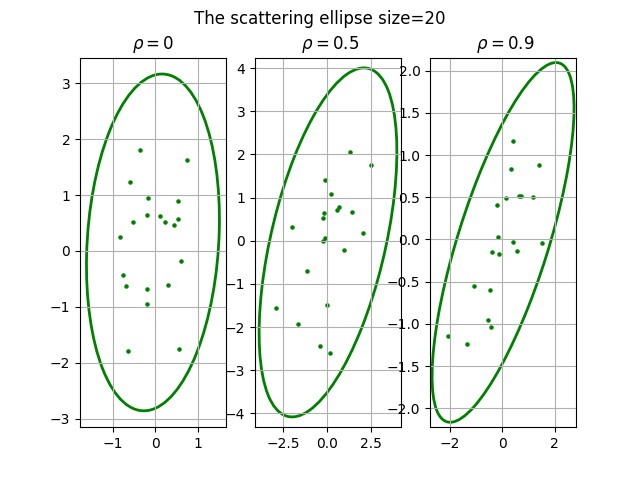
\includegraphics[width = 13cm, height = 8cm]{./lab2_1/pictures/the scattering ellipse size=20.png}
		\caption{Двумерное нормальное распределение, $n$ = 20}
		\label{fig:n20}
	\end{figure}
	
	\begin{figure}[H]
		\centering
		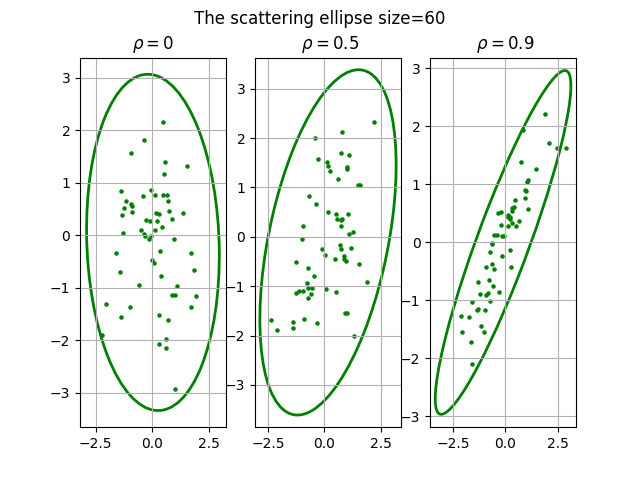
\includegraphics[width = 13cm, height = 8cm]{./lab2_1/pictures/the scattering ellipse size=60.png}
		\caption{Двумерное нормальное распределение, $n$ = 60}
		\label{fig:n60}
	\end{figure}

	\begin{figure}[H]
		\centering
		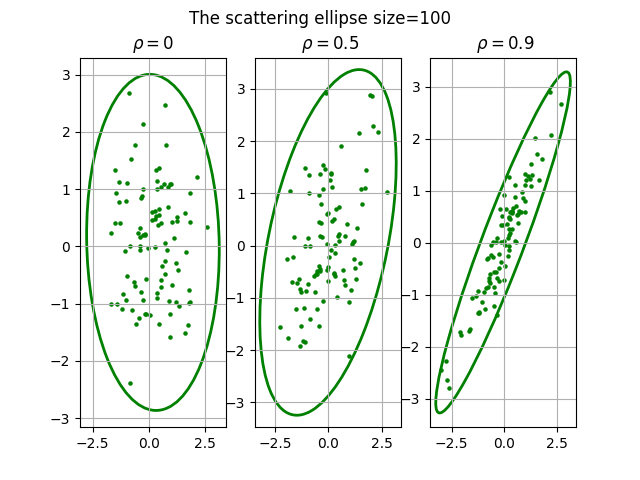
\includegraphics[width = 13cm, height = 8cm]{./lab2_1/pictures/the scattering ellipse size=100.png}
		\caption{Двумерное нормальное распределение, $n$ = 100}
		\label{fig:n100}
	\end{figure}
\subsection{Оценки коэффициентов линейной регрессии}
	
	\noindent Метрика удаленности: $distance = \sum_{i=0}^{n}(y_{model}[i]-y_{regr}[i])^2$
	\subsubsection{Выборка без возмущений}
		\begin{enumerate}
			\item{Критерий наименьших квадратов:}
			$\hat{a}\approx 2.15$, $\hat{b}\approx 1.78$
			\item{Критерий наименьших модулей:}
			$\hat{a}\approx 2.05$, $\hat{b}\approx 1.99$
		\end{enumerate}
		\begin{figure}[H]
			\centering
			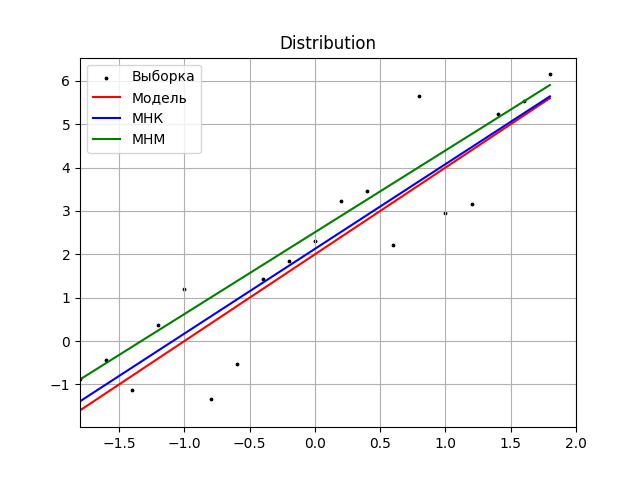
\includegraphics[width = 10cm, height = 8cm]{./lab2_2/pictures/Distribution.png}
			\caption{Выборка без возмущений}
			\label{w/o_pert}
		\end{figure}
	
	\subsubsection{Выборка с возмущениями}
		\begin{enumerate}
			\item{Критерий наименьших квадратов:}
			$\hat{a}\approx 1.88$, $\hat{b}\approx 0.63$
			\item{Критерий наименьших модулей:}
			$\hat{a}\approx 1.63$, $\hat{b}\approx 1.94$
		\end{enumerate}
		\begin{figure}[H]
			\centering
			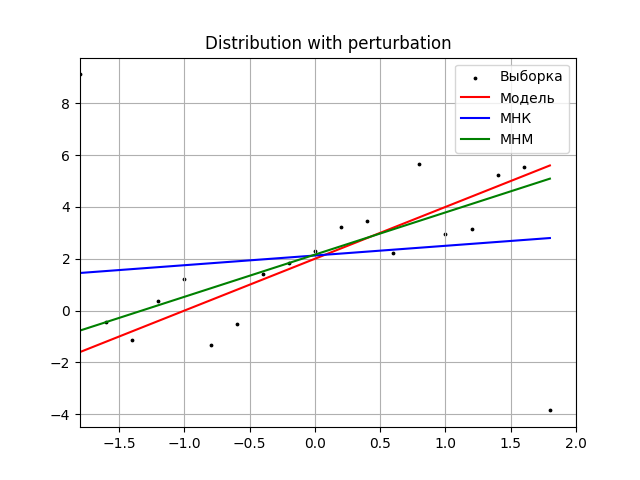
\includegraphics[width = 10cm, height = 8cm]{./lab2_2/pictures/Distribution with perturbation.png}
			\caption{Выборка с возмущениями}
			\label{w_pert}
		\end{figure}
\subsection{Проверка гипотезы о законе распределения генеральной совокупности. Метод хи-квадрат}

\noindent Метод максимального правдоподобия:
\newline
$\hat{\mu} \approx -0.06, \hat{\sigma} \approx 0.92$
\newline
Критерий согласия $\chi^{2}$:
\newline
Количество промежутков $k = 8$
\newline
Уровень значимости $\alpha$= 0.05
\newline
Тогда квантиль $\chi^{2}_{1-\alpha}(k-1)$ = $\chi^{2}_{0.95}(7)$. Из таблицы [3, с. 358] $\chi^{2}_{0.95}(7) \approx 14.07$. 
\begin{table}[H]
	\centering
	\begin{tabular}{| c | c | c | c | c | c | c |}
	\hline
   $i$ & $limits$         &   $n_i$ &    $p_i$ &   $np_i$ &   $n_i - np_i$ &   $\frac{(n_i-np_i)^2}{np_i}$ \\
\hline
   1 & [-inf, -1.1]       &    15 & 0.1357 &  13.5666 &    1.4334 &                0.1514 \\
   2 & [-1.1, -0.73]    &     7 & 0.096  &   9.6012 &      -2.6012 &              0.7047 \\
   3 & [-0.73, -0.37] &    15 & 0.1253 &  12.5256 &       2.4744 &               0.4888 \\
   4 & [-0.37, 0.0]     &    15 & 0.1431 &  14.3066 &       0.6934 &             0.0336 \\
   5 & [0.0, 0.37]      &    11 & 0.1431 &  14.3066 &      -3.3066 &              0.7642 \\
   6 & [0.37, 0.73]   &    13 & 0.1253 &  12.5256 &       0.4744 &              0.018  \\
   7 & [0.73, 1.1]      &    15 & 0.096  &   9.6012 &       5.3988 &              3.0358 \\
   8 & [1.1, 'inf']       &     9 & 0.1357 &  13.5666 &      -4.5666 &              1.5371 \\
   \sum & -                  &   100 & 1      & 100      &      -0      &           6.7338 \\
\hline
\end{tabular}
	\caption{ Вычисление $\chi^{2}_{B}$ при проверке гипотезы $H_{0}$ о нормальном законе распределения $N(x,\hat{\mu}, \hat{\sigma})$}
	\label{tab:normal_chi_2}
\end{table} 

\noindent Сравнивая $\chi^{2}_{B} = 10.19$ и $\chi^{2}_{0.95}(7) \approx 14.07$, видим, что $\chi^{2}_{B} < \chi^{2}_{0.95}(7)$.
\\

\begin{table}[H]
	\centering
	\begin{tabular}{| c | c | c | c | c | c | c |}
		\hline
		$i$ & $limits$         &   $n_i$ &    $p_i$ &   $np_i$ &   $n_i - np_i$ &   $\frac{(n_i-np_i)^2}{np_i}$ \\
		\hline
   1 & [-inf, -1.1]      &     3 & 0.1357 &  2.7133 &       0.2867 &             0.0303 \\
   2 & [-1.1, -0.37]   &     1 & 0.2213 &  4.4254 &      -3.4254 &             2.6513 \\
   3 & [-0.37, 0.37] &    13 & 0.2861 &  5.7226 &       7.2774 &             9.2544 \\
   4 & [0.37, 1.1]     &     3 & 0.2213 &  4.4254 &      -1.4254 &             0.4591 \\
   5 & [1.1, 'inf']      &     0 & 0.1357 &  2.7133 &      -2.7133 &             2.7133 \\
   \sum & -                 &    20 & 1      & 20      &      -0      &          15.1085 \\
\hline
\end{tabular}
	\caption{ Вычисление $\chi^{2}_{B}$ при проверке гипотезы $H_{0}$ о законе распределения $L(x,\hat{\mu}, \hat{\sigma})$, $n=20$}
	\label{tab:laplace_chi_2}
\end{table}
\noindent Сравнивая $\chi^{2}_{B} = 8.19$ и $\chi^{2}_{0.95}(4) \approx 9.49$, видим, что $\chi^{2}_{B} < \chi^{2}_{0.95}(4)$.

\begin{table}[H]
	\centering
	\begin{tabular}{| c | c | c | c | c | c | c |}
	\hline
		$i$ & $limits$         &   $n_i$ &    $p_i$ &   $np_i$ &   $n_i - np_i$ &   $\frac{(n_i-np_i)^2}{np_i}$ \\
	\hline
  1 & [-inf, -1.1]      &     4 & 0.1357 &  2.7133 &       1.2867 &                 0.6102 \\
   2 & [-1.1, -0.37]   &     8 & 0.2213 &  4.4254 &       3.5746 &               2.8875 \\
   3 & [-0.37, 0.37] &     3 & 0.2861 &  5.7226 &      -2.7226 &              1.2953 \\
   4 & [0.37, 1.1]     &     4 & 0.2213 &  4.4254 &      -0.4254 &              0.0409 \\
   5 & [1.1, 'inf']      &     1 & 0.1357 &  2.7133 &      -1.7133 &              1.0819 \\
   \sum & -                 &    20 & 1      & 20      &      -0      &           5.9157 \\
\hline
	\end{tabular}
	\caption{ Вычисление $\chi^{2}_{B}$ при проверке гипотезы $H_{0}$ о законе распределения $U(x,\hat{\mu}, \hat{\sigma})$, $n=20$}
	\label{tab:uniform_chi_2}
\end{table}

\noindent Сравнивая $\chi^{2}_{B} = 5.67$ и $\chi^{2}_{0.95}(4) \approx 9.49$, видим, что $\chi^{2}_{B} < \chi^{2}_{0.95}(4)$.

\subsection{Доверительные интервалы для параметров нормального распределения}
    \begin{figure}[H]
		\centering
		    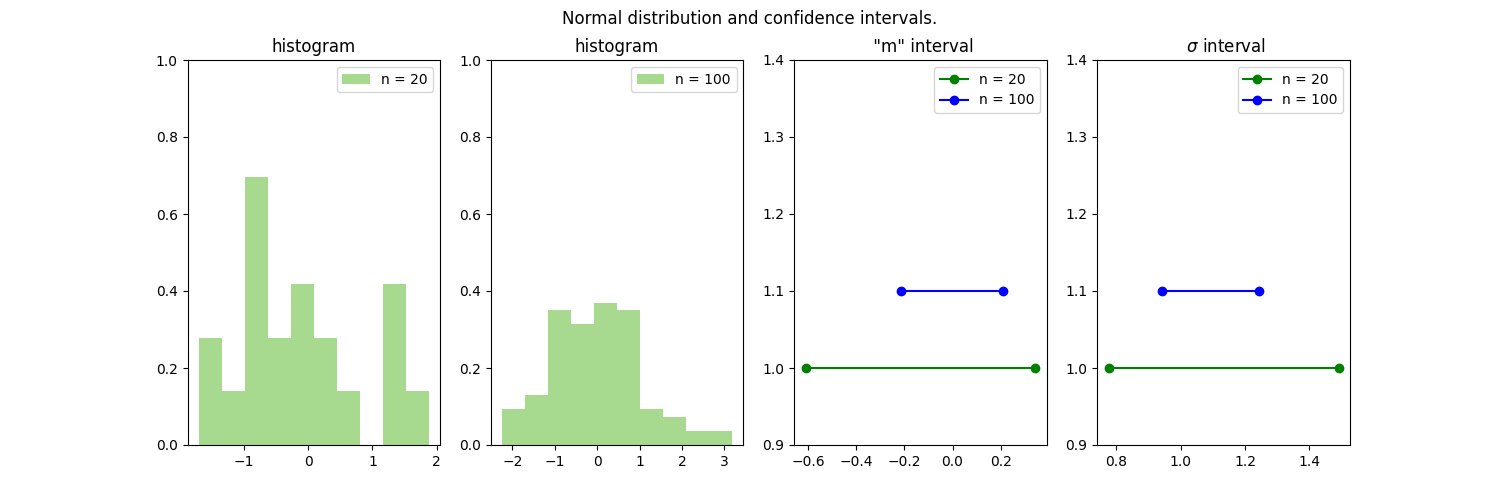
\includegraphics[width = 18cm, height = 6cm]{./lab2_4/pictures/norm.png}
		\caption{Гистограммы нормальных распределений и доверительные интервалы их параметров}
		\label{w_pert}
	\end{figure}
		
	\begin{table}[H]
	    \centering
	    \begin{tabular}{| c | c | c |}
	    \hline
	       n = 20   &  $m$  & $\sigma$\\ \hline
	          &  -0.61 < $m$ < 0.34 & 0.78 < $\sigma$ < 1.49 \\ \hline
	         &   &   \\ \hline
	       n = 100   &  $m$  & $\sigma$\\ \hline
	        & -0.21 < $m$ < 0.21 & 0.94 < $\sigma$ < 1.24 \\
	   \hline
	    \end{tabular}
	    \caption{Доверительные интервалы для параметров нормального распределения}
	    \label{tab:interv_simple}
	\end{table}
	
\subsection{Доверительные интервалы для параметров произвольного распределения. Асимптотический подход}
    \begin{figure}[H]
		\centering
			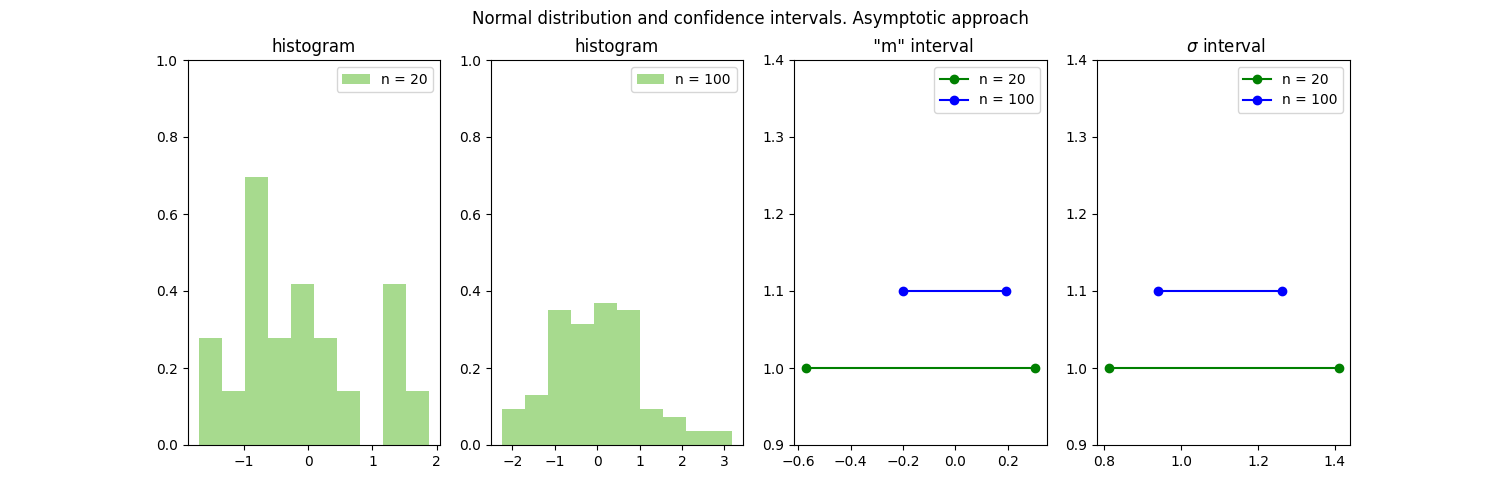
\includegraphics[width = 18cm, height = 6cm]{./lab2_4/pictures/asymp.png}
		\caption{Гистограммы нормальных распределений и доверительные интервалы их параметров. Асимптотический подход}
		\label{w_pert}
	\end{figure}
	
	\begin{table}[H]
	    \centering
	    \begin{tabular}{| c | c | c |}
	    \hline
	       n = 20   &  $m$  & $\sigma$\\ \hline
	          &  -0.57 < $m$ < 0.3 & 0.81 < $\sigma$ < 1.41 \\ \hline
	         &   &   \\ \hline
	       n = 100   &  $m$  & $\sigma$\\ \hline
	        & -0.2 < $m$ < 0.19 & 0.94 < $\sigma$ < 1.26 \\
	   \hline
	    \end{tabular}
	    \caption{Доверительные интервалы для параметров произвольного распределения. Асимптотический подход}
	    \label{tab:interv_asimpt}
	\end{table}
\section{Обсуждение}
\subsection{Выборочные коэффициенты корреляции}
\noindent Для двумерного нормального распределения дисперсии выборочных коэффициентов корреляции упорядочены следующим образом: $r < r_{S} < r_{Q}$; для смеси распределений получили обратную картину: $r_{Q} < r_{S} < r$.
\newline
\noindent Процент попавших элементов выборки в эллипс рассеивания (95$\%$-ная доверительная область) примерно равен его теоретическому значению (95$\%$).
\subsection{Оценки коэффициентов линейной регрессии}
\noindent По полученным результатам можно сказать, что критерий наименьших квадратов точнее оценивает коэффициенты линейной регрессии на выборки без возмущений. Если же редкие возмущения присутствуют, тогда лучше использовать критерий наименьших модулей, поскольку он более устойчив.
\subsection{Проверка гипотезы о законе распределения генеральной совокупности. Метод хи-квадрат}
	
\noindent Заключаем, что гипотеза $H_{0}$ о нормальном законе распределения $N(x,\hat{\mu}, \hat{\sigma})$ на уровне значимости $\alpha = 0.05$ согласуется с выборкой для нормального распределения $N(x, 0, 1)$.
\\
Также видно, что для выборок сгенерированных по равномерному закону и закону Лапласа гипотеза $H_{0}$ оказалась принята.
 \subsection{Доверительные интервалы для параметров распределения}
 \begin{itemize}
    \item Генеральные характеристики ($m$ = 0 и $\sigma$ = 1) накрываются построенными доверительными интервалами. 
    \item Также можно сделать вывод, что для большей выборки доверительные интервалы являются соответственно более точными, т.е. меньшими по длине. 
    \item Кроме того, при большом объеме выборки асимптотические и классические оценки практически совпадают.
\end{itemize}

\end{document}